\chapter{LinkedPipes Visualization}

We already gave a brief description of LinkedPipes Visualization \cite{linked_pipes_visualization} at the end of the previous chapter. The authors state: \emph{"You point LinkedPipes Visualization to the data and it tells you what it sees in it. This way, you get to a visualization in just a few clicks."}  \cite{linked_pipes_visualization}. We will use this tool as a base for our \emph{application generator}. We will turn \emph{visualizations} into configurable interactive \emph{applications} which will push the whole concept to the next level. Before we get to how we want to achieve that and especially why we decided to use LinkedPipes Visualization in the first place, we will give the reader a deeper and more profound description of this tool. This knowledge will be required in the later parts of this text.

LinkedPipes Visualization implements the Linked Data Visualization Model. We start by describing this model as a concept, then we move on to the description of how LinkedPipes Visualization implements this model. The following section is dedicated to features of this tool in general, i.e., what it is capable of. The chapter is concluded with more technical information and implementation details of LinkedPipes Visualization.

\section{LDVM}

Linked Data Visualization Model (LDVM) \cite{ldvm} is an abstract concept that breaks down the visualization process of Linked Data into four separated stages. Those stages are \emph{Source Data}, \emph{Analytical Abstraction}, \emph{Visualization Abstraction} and \emph{View} [cite ldvm]. Let us walk through the individual stages.

\begin{itemize}
\item In the \emph{Source Data} stage, we begin with raw input data in an arbitrary format (it can but does not have to be in RDF). In this stage appropriate transformations need to be applied on the input data to convert them into RDF representation suitable for the next stage. For example, a CSV file could be converted into corresponding RDF representation at this stage. If the input data already are in RDF, this stage could be reduced to simple identity mapping. This transformation is done by a component which is called a \emph{data source}.
\item In the \emph{Analytical Abstraction} stage, relevant data are extracted and represented from the input produced in the \emph{Source Data} stage. Also arbitrary aggregation and computation of additional characteristics can be performed at this stage. This is typically done through a sequence of in-stage SPARQL operators. This sequence is denoted as an \emph{analyzer} component.
\item In the \emph{Visualization Abstraction} stage, the \emph{analytical abstraction} produced by the previous stage is transformed into \emph{visualization abstraction} which corresponds to the desired visualization technique. Under the hood it works very similarly to the \emph{analytical abstraction} stage as the transformation is also achieved through a sequence of in-stage SPARQL operators which is denoted as an \emph{visualization transformer} component.
\item In the final \emph{View} stage, the \emph{visualization abstraction} is transformed into an actual on-screen visualization that the user can see and potentially interact with. This visual mapping transformation is performed by a component called \emph{visualizer}.
\end{itemize}

By putting this all together, we get a \emph{pipeline} which on one end takes some arbitrary data as an input, and on the other end produces an actual on-screen visualization of the input data. If we look closely at the \emph{pipeline}, it starts with transforming the data into RDF, then follows a sequence of SPARQL operators and finally it ends with the visualization. The reason why the process is abstracted into four separate stages with four separate types of components is re-usability and composability. 

\subsection{Combining and re-using components}

Let us say we have a data set that contains a list of cities,  their populations and the countries they belong to. Clearly, all kinds of information can be extracted from such a data set. We might want to select just the cities. Or we might want to select the countries and calculate the number of cities in each country. Or we might want to select the countries and calculate the average population size of all cities in a country. For each of these tasks we would define a different \emph{analyzer}.

Now let us say we have the list of the cities and we want to visualize them on a map. Each city has GPS coordinates attached to it but unfortunately, it is using a vocabulary that our map \emph{visualizer} does not understand. In this case, we can use a \emph{visualization transformer} that converts the geospatial information into the desired format by using the supported vocabulary.

Eventually, we might have two different map \emph{visualizers} available, one is Google Maps based and the other one is OpenStreetMap based. Both can work with the output of the earlier mentioned \emph{visualization transformer}. Therefore, the user can choose which one suits his need best.

The final pipeline in this example might consist of the \emph{data source}, the \emph{analyzer} that extracts the cities, the \emph{visualization transformer} that converts the geospatial information to the supported format, and eventually the \emph{visualizer} that shows the selected cities on a map.

What is important here is that every single component in this pipeline can be re-used and based on the context, it can yield different results. All kinds of other information can be extracted from this \emph{data source}. This particular \emph{analyzer} can extract cities from different \emph{data sources} and pass them on. We can easily imagine that the task of converting the geospatial data between two vocabularies, which is what our \emph{visualization transformer} does, will be pretty common. Finally, the map \emph{visualizer} can be used to visualize any geospatial data.

\subsection{Compatibility}

On top of all of this, LDVM introduces a very important concept of \emph{compatibility}. \emph{Analyzers}, \emph{visualization transformers} and \emph{visualizers} are software components that consume data through their input interfaces. What we want to know is whether an \emph{analyzer} can be applied on a \emph{data source}, whether a \emph{visualization transformer} can be applied on an \emph{analytical abstraction} and whether a \emph{visualizer} can visualize a \emph{visualization abstraction}. To achieve this, the concept of \emph{compatibility} requires that every LDVM component describes the expected format of the input data using an \emph{input signature}. The implementation details of an \emph{input signature} are not important at this moment. What matters is that thanks to \emph{input signatures} we can automatically check the \emph{compatibility} of two LDVM components, i.e., whether the output of one component can be \emph{bound} to the input of another component.

If we look back at Payola, there are many similar aspects. A Payola \emph{analysis} is also a pipeline that consists of connected \emph{plugins} that somehow process and transform the RDF data. However, there is no such thing as \emph{compatibility} in Payola. It is the user who needs to check that it is possible to combine two plugins together.

The concept of \emph{compatibility} in LDVM has two big consequences. Firstly, it is possible to automatically check that a created pipeline makes sense and can work. Secondly, it is actually possible to automatically generate a pipeline from given \emph{data source} using available LDVM components. We will describe this more in detail in the next section.

\section{LDVM implementation}

The implementation of LDVM in LinkedPipes Visualization \cite{ldvm_use_cases} uses those exact four types of components defined by the model. Each component can have multiple inputs and a single output. An exception are the \emph{data source} components that have no inputs and \emph{visualizer} components that have no output. 

\subsection{Features and input descriptors}

To support compatibility, each component defines a set of its \emph{features}, where each feature corresponds to a part of expected component functionality. Using \emph{input descriptors}, a feature can define what kind of data it requires in order to be used. The implementation distinguishes between \emph{mandatory} features and \emph{optional} features. In order for two components to be considered \emph{compatible}, the output of the first component must meet the requirements defined by \emph{input descriptors} of all \emph{mandatory features} of the second component.

Let us say that we have a map \emph{visualizer} with two \emph{features}. The first \emph{feature} represents the ability to display points on a map, the second one represents the ability to show labels of those points. The first one is \emph{mandatory} because without it,  we would have clearly nothing to visualize. The second one, on the other hand, can be left as \emph{optional} because without it, we still have something to show on the map. We borrowed this exact example from \cite{ldvm_use_cases}. 

Now, if we want to check the \emph{compatibility} between this \emph{visualizer} and (typically) a \emph{visualization transformer}, i.e., we want to check whether it is possible to bind the output of the \emph{visualization transformer} to the input of the map \emph{visualizer}, we can check the data produced by the \emph{visualization transformer} against the \emph{input descriptor} of the \emph{mandatory feature} to get that information. In simple words: The \emph{mandatory feature} in our example represents the ability to display points on a map. So this feature requires the input data to contain some points that can be visualized on a map. This requirement is expressed using the \emph{feature's input descriptor}, i.e., the \emph{input descriptor} says that the input data need to contain such points. So checking the \emph{compatibility} in this case actually means checking whether the output of \emph{visualization transformer} contains some points.

\subsection{Output data samples}

The last sentence in the previous paragraph suggests that in order to ensure the \emph{compatibility}, it is necessary to \emph{run} the \emph{pipeline} (i.e., apply all the SPARQL operators from all LDVM components in a pipeline on the input data) so that we get the actual data at each stage and can apply the \emph{input descriptors} on them. As the input data might be fairly large, the process of building a \emph{pipeline} could take very long.

To address this issue, the LDVM implementation in LinkedPipes Visualization requires \emph{analyzers} and \emph{visualization transformers} to provide besides the \emph{input descriptors} also an \emph{output data sample}. In order to work properly, the \emph{output data sample} should resemble the actual output of this particular component, but it should be as small as possible. For example, if an \emph{analyzer} produces a list of cities with their population, the \emph{data sample} should contain only one city (but with all information related to that one city). When checking the compatibility, the \emph{input descriptors} are applied on the \emph{output data sample} instead of the actual output of the previous component. That means that we do not need to run the \emph{pipeline} in order to check the compatibility. As the \emph{output data sample} is small, this checking should be fast.

Thanks to this approach, the \emph{compatibility} can be quickly checked at the design time and when we decide to \emph{run} the \emph{pipeline}, we can already be sure that all the components are at least compatible between each other.

\subsection{Component representation}

To follow the Linked Data principles, LinkedPipes Visualization implementation of LDVM represents the  components and their configuration in RDF using a custom RDF vocabulary prefixed with \texttt{ldvm} \cite{ldvm_vocabulary}. That makes it possible for the LDVM components to be shared and exchanged with separate instances of LinkedPipes Visualization or possibly even with completely different LDVM based software that supports this RDF representation. This is, however, true only to an extent. Some of the components are truly transferable and independent on the actual software implementation, but many of them require to have a corresponding counterpart in the programming code. This applies to \emph{visualizers} (the tool actually needs to implement the visualization technique required by the \emph{visualzer} component) but also to some \emph{analyzers} or \emph{transformers} for which simple SPARQL operators are not sufficient.

\subsection{Discovery}

Finally, we get to the most important feature and that is automatic \emph{pipeline discovery}. LinkedPipes Visualization maintains a register of available LDVM components: \emph{data sources}, \emph{analyzers}, \emph{visualization transformers} and \emph{visualizers}. We can think of this register as of a \emph{graph}, where each component is a vertex and two components are connected by a directed edge if and only if they are \emph{compatible}. What LinkedPipes Visualization allows us to do is to select some \emph{data sources} (or add new ones). Then, it will automatically \emph{discover} (using an algorithm similar to Breadth-first search) all possible pipelines that start with selected \emph{data sources} and end with one of the available \emph{visualizers}. Note that a \emph{pipeline} is a hierarchical structure. As components can have multiple inputs, it is possible to combine the data from multiple \emph{data sources}.

\section{Features}

\subsection{Discovering visualizations}

From a \emph{non-developer} user perspective, LinkedPipes Visualization is a tool for quick and automatic visualization of arbitrary RDF data. The user simply selects a data source (or multiple data sources) and the tool returns him a list of discovered \emph{pipelines}. Each \emph{pipeline} is ended with a \emph{visualizer} which probably is the actual information that the \emph{non-developer} user is interested in. He selects one of the \emph{pipelines} and \emph{runs} it which will process all the input data according to the component definitions and finally it will produce data ready to be consumed by the \emph{visualizer}. Once this is done, the user is redirected to the actual \emph{visualization} of the produced data using the selected \emph{visualizer} component. Each such \emph{visualization} lives at a unique URL which means that it can be accessed later or shared with other users.

\begin{figure}
	\centering
	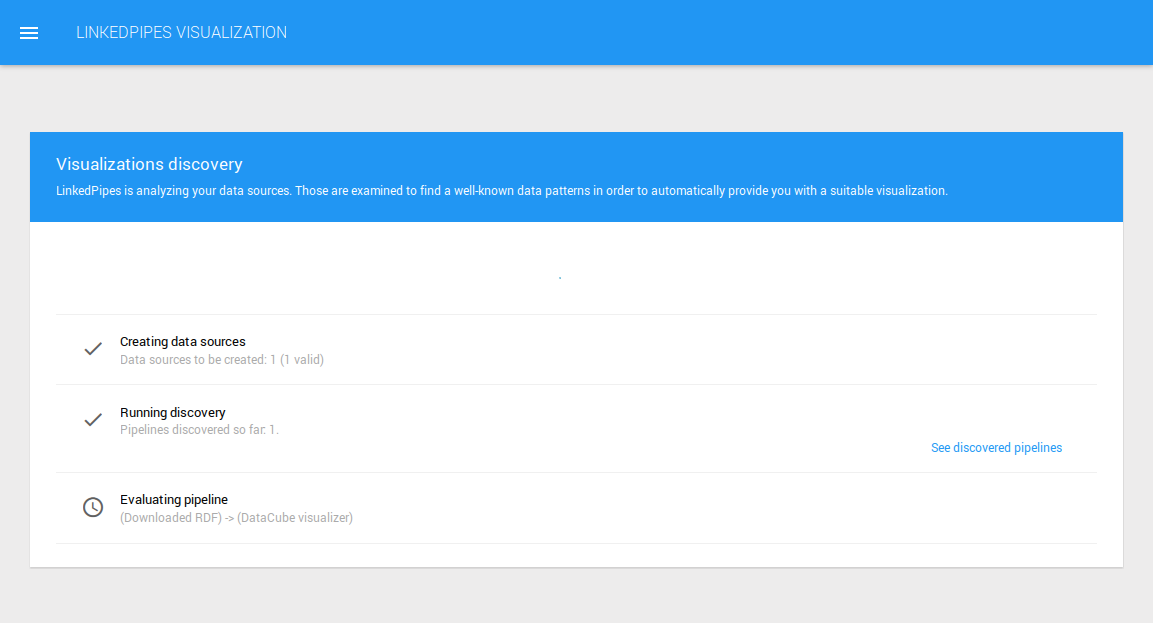
\includegraphics[width=130mm]{img/03_linked_pipes_discovery.png}
	\caption{Discovery progress in LinkedPipes Visualization} 
	\label{fig:linked-pipes-discovery}
\end{figure}

It is worth mentioning that the LinkedPipes Visualization can accept the source RDF data in many forms. It can be a SPARQL endpoint, it can be a URL pointing to a file containing RDF data serialized in one of the existing formats (TTL, RDF/XML etc.) or such a file can be directly uploaded to LinkedPipes Visualization. As already mentioned, non-RDF data are not supported.

\subsection{Adding components}

More advanced users that understand RDF on a lower technical level and are capable of writing SPARQL queries, can implement and add their own LDVM components. A typical scenario might be that such a user has a new RDF data set and he wants to use one of the available \emph{visualizers} to visualize it. To achieve that, he can develop his own LDVM component, an \emph{analyzer} or \emph{visualization transformer} (or both), that converts the input data set into the format required by the \emph{visualizer}. The definition of such a component can be easily uploaded through LinkedPipes Visualization user interface. Once this is done, the new component becomes part of the register and can be used by the \emph{discovery algorithm}.

\begin{figure}
	\centering
	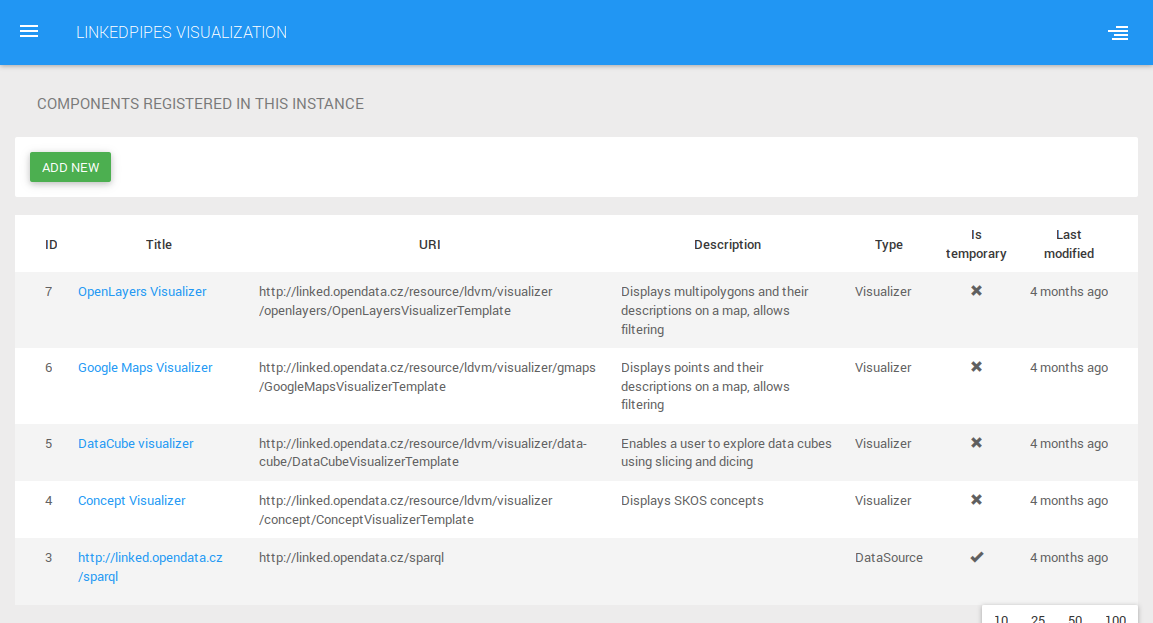
\includegraphics[width=130mm]{img/03_linked_pipes_components.png}
	\caption{Overview of available registered LDVM components in LinkedPipes Visualization} 
	\label{fig:linked-pipes-components}
\end{figure}

Users with actual developer skills can extend LinkedPipes Visualization with new \emph{visualizers} and more advanced \emph{analyzers} and \emph{visualization transformers}. That involves developing both the RDF definition using the \texttt{ldvm} vocabulary and the corresponding counterpart in programming code. 

\section{Implementation}

In the next section we will give the reader an overview of the inner architecture and used technologies. We will especially focus on how \emph{visualizers} work as those will essentially be our \emph{generated applications}.

\subsection{Architecture}

LinkedPipes Visualization is a web application that consists of a backend running on a server and a frontend running on the client side (in a web browser). 

The frontend is a so called Single-page application (SPA). That means that the application user interface lives completely in the browser and uses asynchronous HTTP requests (AJAX) to communicate with the backend. The data between the server and the client are sent serialized to JSON.

To be more accurate, LinkedPipes Visualization actually consists of several SPAs, each dealing with a different task. Visualization is one SPA, component management is one SPA and each visualizer is also one SPA. The frontend is driven by the JavaScript framework AngularJS and the interface is created using modern web technologies, specifically HTML5 and CSS3. Several other JavaScript libraries are used as well (for example D3.js for creating rich visualizations).

The backend is developed in Scala using Play Framework. This framework follows MVC architecture, nevertheless in this case the \emph{View} layer is significantly suppressed as its work is done by the thick client. The tool uses H2 relational database to persist arbitrary application data, and the triplestore Virtuoso as a private RDF data storage (that is required, for example, when evaluating \emph{pipelines}). 

\subsection{Component registration}

We mentioned that if the user uploads a definition of a new LDVM component, its added to the \emph{register}. What actually happens under the hood is that such a component gets inserted into the H2 database where it can be easily accessed during the \emph{discovery}. We also mentioned that some LDVM components require their counterparts directly in the code.

Let us start with \emph{analyzers} and \emph{visualization transformers}. These components perform transformations on the RDF data. Typically, this is done using SPARQL operators but sometimes that is not enough and the transformation needs to be implemented using an actual programming language (Scala in this case). The backend code contains a simple \texttt{switch} that defines which snippet of code should be executed for which component (the \emph{snippet} is actually a well-defined \emph{plugin} implementing given plugin interface). Here we would like to remind the reader that components are defined and represented in RDF using the \texttt{ldvm} vocabulary. That means that each component is actually an RDF resource with a unique URI. This URI is used in the \texttt{switch} to identify the components. 

So if a user wants to create such a component, firstly, he needs to create the RDF definition of that component and upload it, secondly, he needs to develop the plugin doing the actual component work (the data transformation), and lastly, he needs to add the component to the aforementioned \texttt{switch}. 

The situation is very similar for \emph{visualizers} as well. Each visualizer is a standalone SPA that lives on a unique URL. When the evaluation of a \emph{pipeline} finishes, the user needs to be redirected to this URL. So just as there is a \texttt{switch} defining which plugin corresponds to which \emph{analyzer} (or \emph{visualizer}), there is a \texttt{switch} defining which URL corresponds to which \emph{visualizer} (a \emph{visualizer component} is also identified by a URI).

\subsection{Visualizers}

As already explained, a \emph{visualizer} is a standalone SPA that lives on a unique URL within LinkedPipes Visualization web application. Part of this URL is a parameter which specifies the \emph{pipeline} output that should be visualized using this \emph{visualizer}. The output (or more correctly the \emph{pipeline evaluation}) is a named graph stored in the private triplestore. Each \emph{pipeline evaluation} is also represented by a record in the H2 database and this record contains the graph name. The numeric \texttt{id} of this record is passed through the aforementioned URL parameter. We can say, in this sense, that a \emph{visualizer} is a function that takes the \emph{pipeline evaluation} \texttt{id} as an argument and returns the actual \emph{visualization}.

A typical workflow of a \emph{visualizer} is that once the SPA is loaded, it starts making asynchronous HTTP requests to the backend to fetch the data that should be visualized. The requests are translated by controllers into API calls to the \emph{Model} layer.  The \emph{Model} layer converts API calls into SPARQL queries that fetch data from the named graph which is stored in the private triplestore and contains the \emph{pipeline evaluation}. The returned RDF data are extracted into a representation of native Scala objects and eventually converted to JSON and sent back to the client where they are visualized for the user.

The \emph{pipeline evaluation} might be too large or it still might not be in the proper format for the chosen visualization technique. It is a responsibility of a \emph{visualizer} to deal with these potential problems and that might require some more transformations along the way. Those can be done both on the client side and the server side, whichever way is more suitable. It is not always possible to send the whole data set directly to the client and it has to be somehow reduced on the server side. A typical example of such reduction is that the \emph{visualizer} lets the user apply some filters first. That means that it (ideally) never fetches (and visualizes) the whole data set at once but always only a subset specified by the user. 